\documentclass[12pt]{book}
\usepackage{graphicx}
\usepackage[utf8]{inputenc}
\usepackage{hyperref}
\usepackage[intlimits]{amsmath}
\usepackage{amssymb}
\pretolerance=2000
\tolerance=3000
\renewcommand{\figurename}{Figura}
\renewcommand{\chaptername}{Cap\'{i}tulo}
\renewcommand{\contentsname}{\'{I}ndice}
\renewcommand{\tablename}{Tabla}
\renewcommand{\bibname}{Bibliograf\'{i}a}
\renewcommand{\appendixname}{Ap\'endices}


\title{Riemann problem}
\date{}
\begin{document}
\section*{Results}

Without losing generality we can consider rhoLeft greater than rhoRight otherwise the graphic will be reversed 
(the shock wave moving to the left, the rarefaction wave moving to the right, and the velocity with inversed sign)

\begin{figure}[!h]
 \centering
 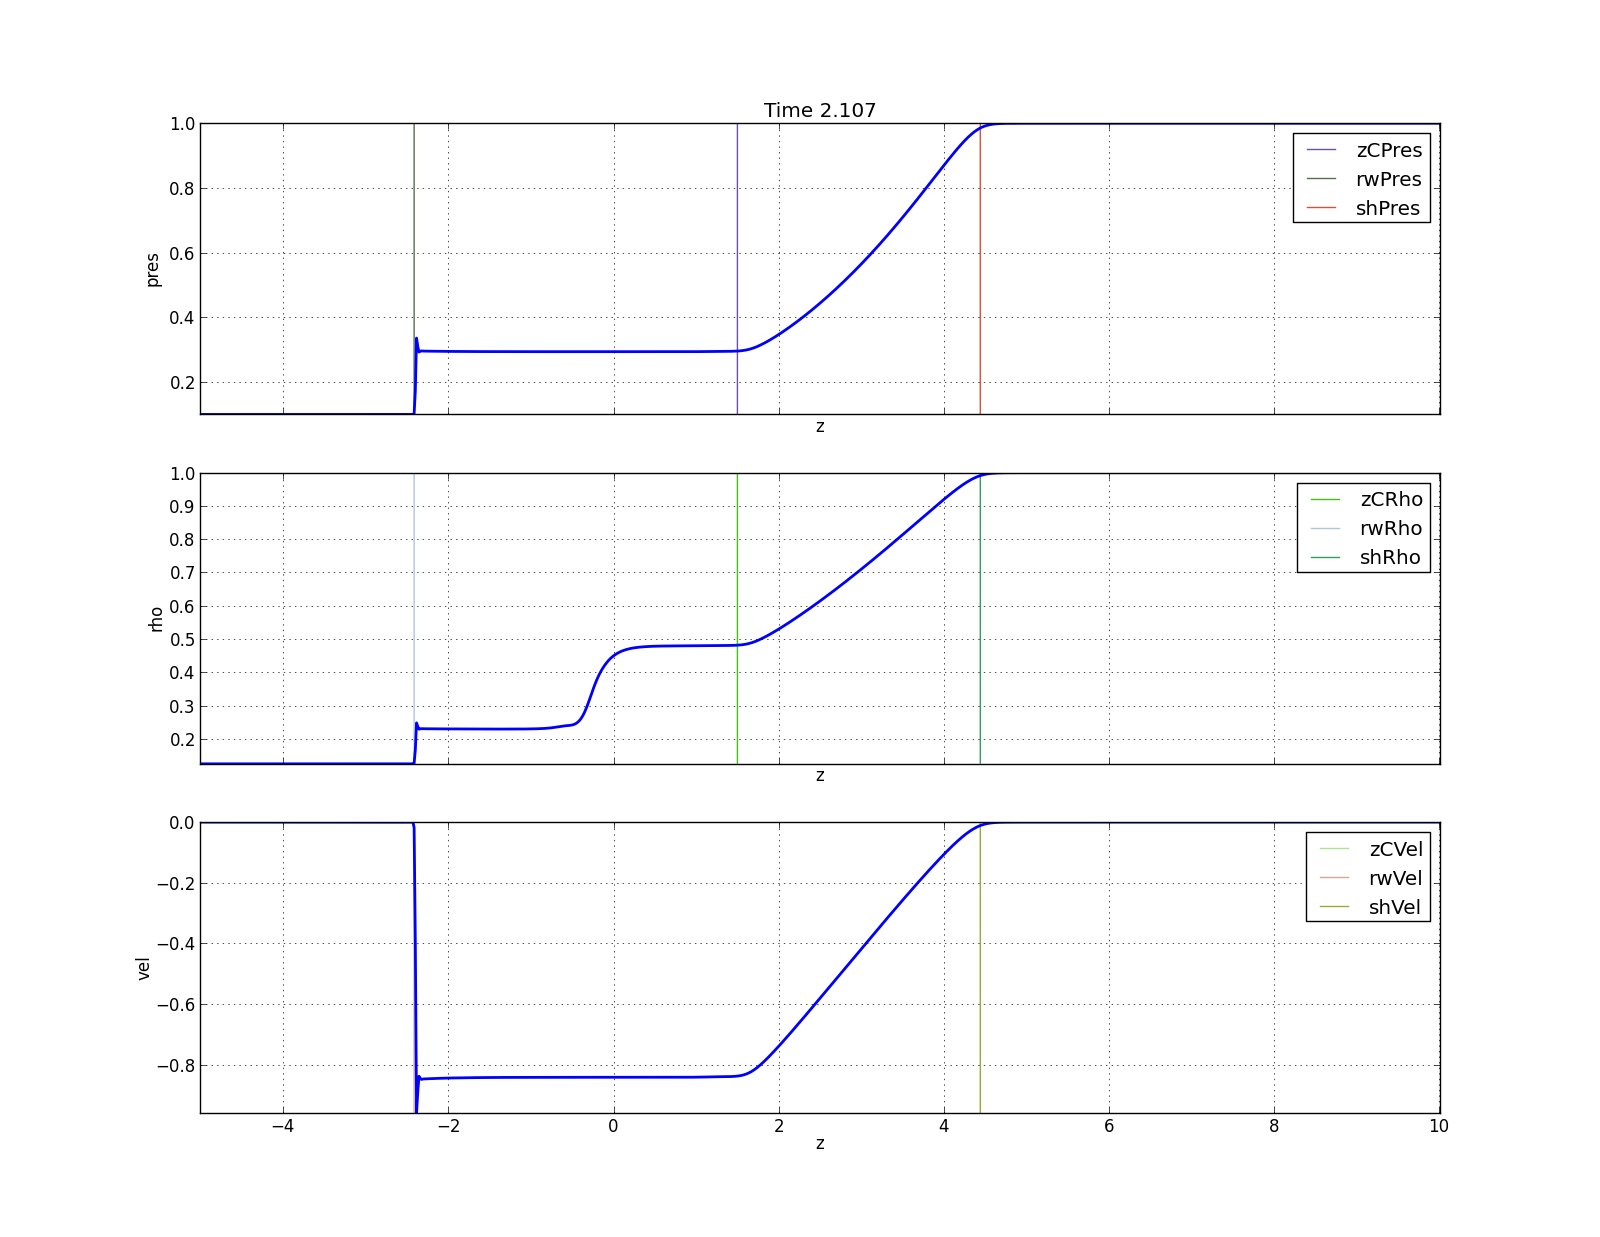
\includegraphics[scale=0.4]{reverse.png}
	\caption{\emph{shock tube reversed}}
 \label{Fig: 1}
\end{figure}

From now on we olly consider cases when shock wave is moving left and rw left(it's checked in initcond\_riemann for rho1 \textgreater rho2) 

The points in the task file : p1, p2, p3, p4, p5, p6
Obs:
\begin{enumerate}
	\item pres1 = presRight
	\item rho1 = rhoRight
	\item vel1 = velRight
	\item vel2 = vel3
	\item pres2 = pres3
	\item pres6 = presLeft
	\item vel6 = velLeft
	\item rho6 = rhoLeft
	\item in the discontinuity part (p2-p3) density is not constant, dcPoint will mark where it changes(it's discontinuous) rho2 \textless rho1
	
\end{enumerate}

\begin{enumerate}
\item rwPoint and shPoint are determned empirically(taking the points from left, right respective when the function pressure is not constant anymore) - analyze\_functions.py
\item The rarefaction wave is moving  with speed(csRW) velLeft - csLeft and rwPoint is also plotted like this (rwPointAn in the graphic: Point is Rho, Pres and Vel). The point is initialized with the value of rwPoint after the time = timeAfterAnPoints (defined in riemann\_params.py)
\item When velLeft = velRight = 0(not in the case of complete problem) the shock wave is moving  with speed(csShock) vel2 * rho2 / (rho2 - rhoRight) in the graphic marked as shPointAn
initialized in the same way as rwPointAn(after timeAfterAnPoints)
\item dcPoint is moving with speed vel2 and it's initialized at the beginning = zC(it is analytically calculated. here analytically means that it was calculated and not empirically determined by observing the shaoes of the functions )
\item the expressions from tasks file are evaluated after timeAfterAnPoints so we should redirect output
\begin{verbatim}
python main.py --timeEnd=10 > out
\end{verbatim}
The output for the paramers in tasks file is in files out\_*
\item We can mark point p1, p2, p3, p4, p5, p6 - (set mark6Points to True in model\_riemann.py) to see where actually the values are calculated - they are points right /and left of shPoint, zC, and rwPoint respectivelly
(we can change them (moving them closer or farther) by changing  delta  in checkExpressions function in model\_riemann.py

\end{enumerate}
\section*{Shock tube}

\begin{figure}[!h]
 \centering
 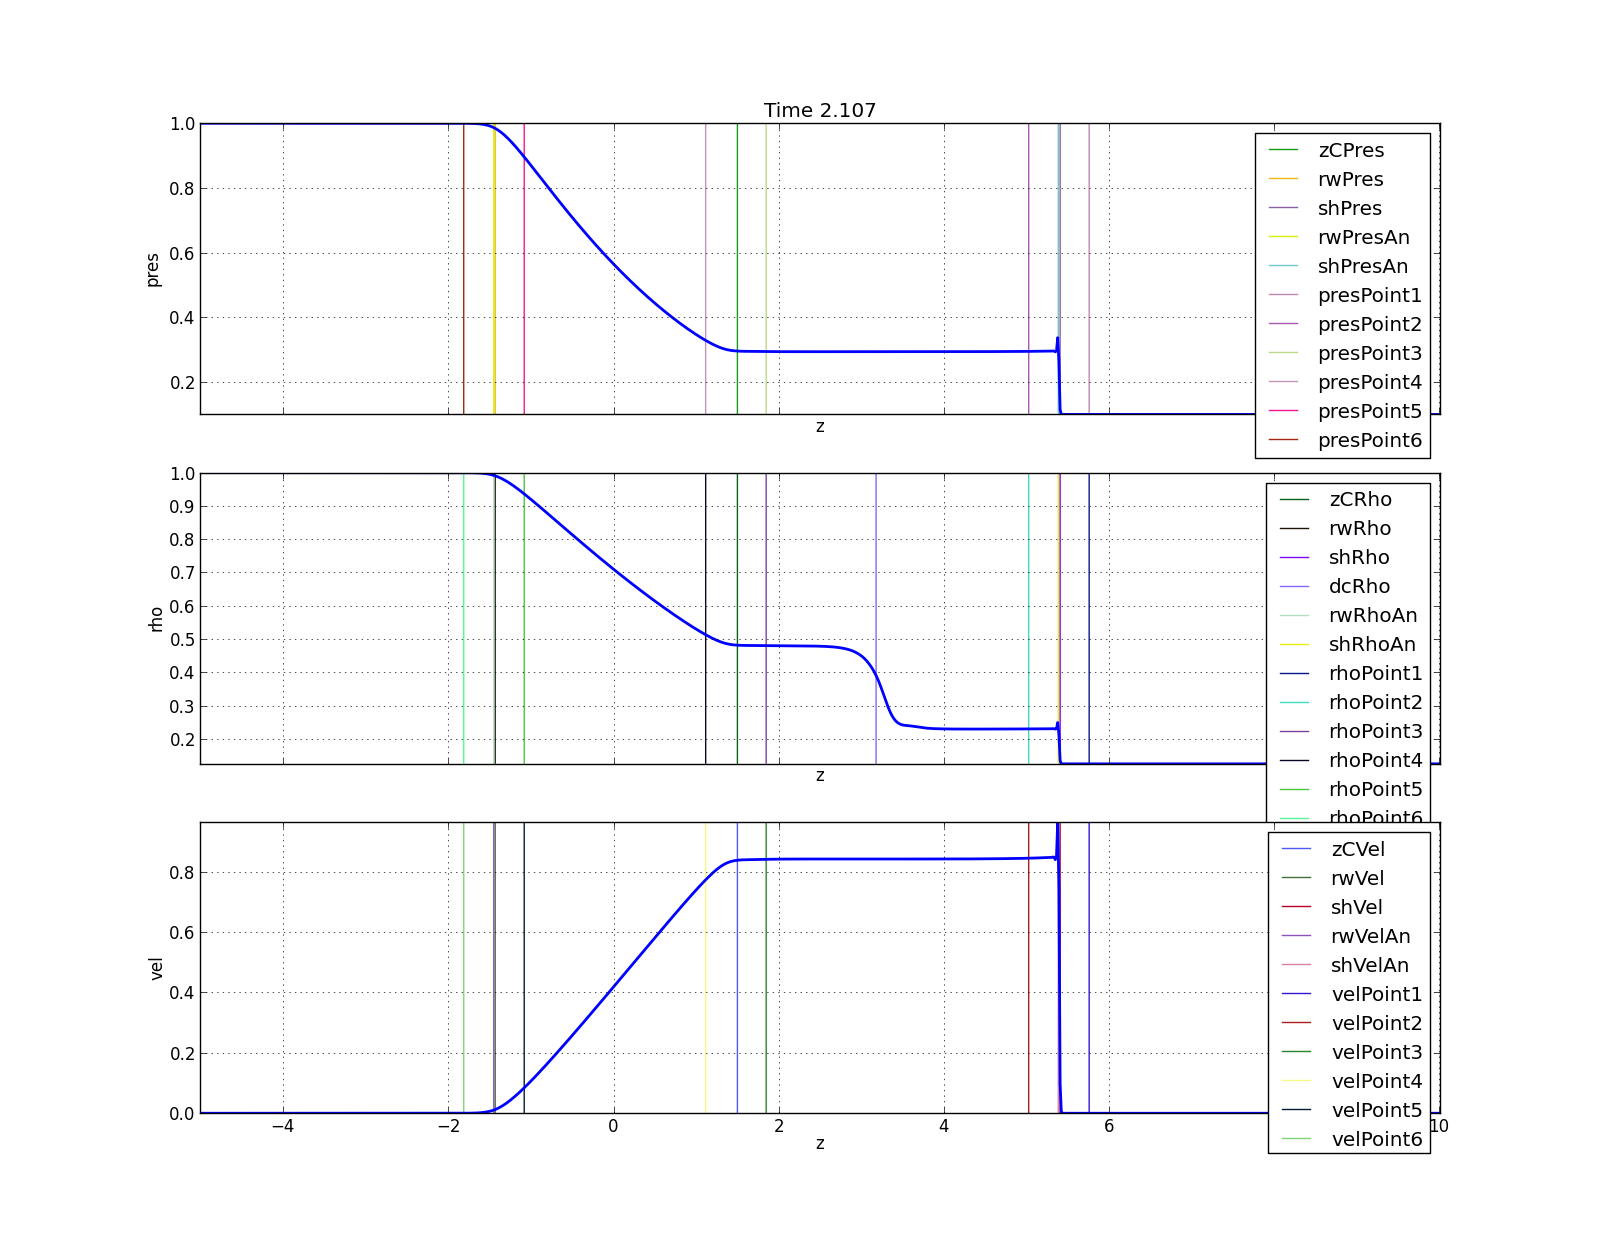
\includegraphics[scale=0.4]{shocktube.png}
	\caption{\emph{shock tube}}
 \label{Fig: 1}
\end{figure}


Observations:
\begin{enumerate}
\item cs6 = -csRW
\item csShock \textgreater cs1 and csShock \textgreater cs2
\item relations fulfilled see out\_shocktube file
\end{enumerate}


\section*{Complete}

\begin{figure}[!h]
 \centering
 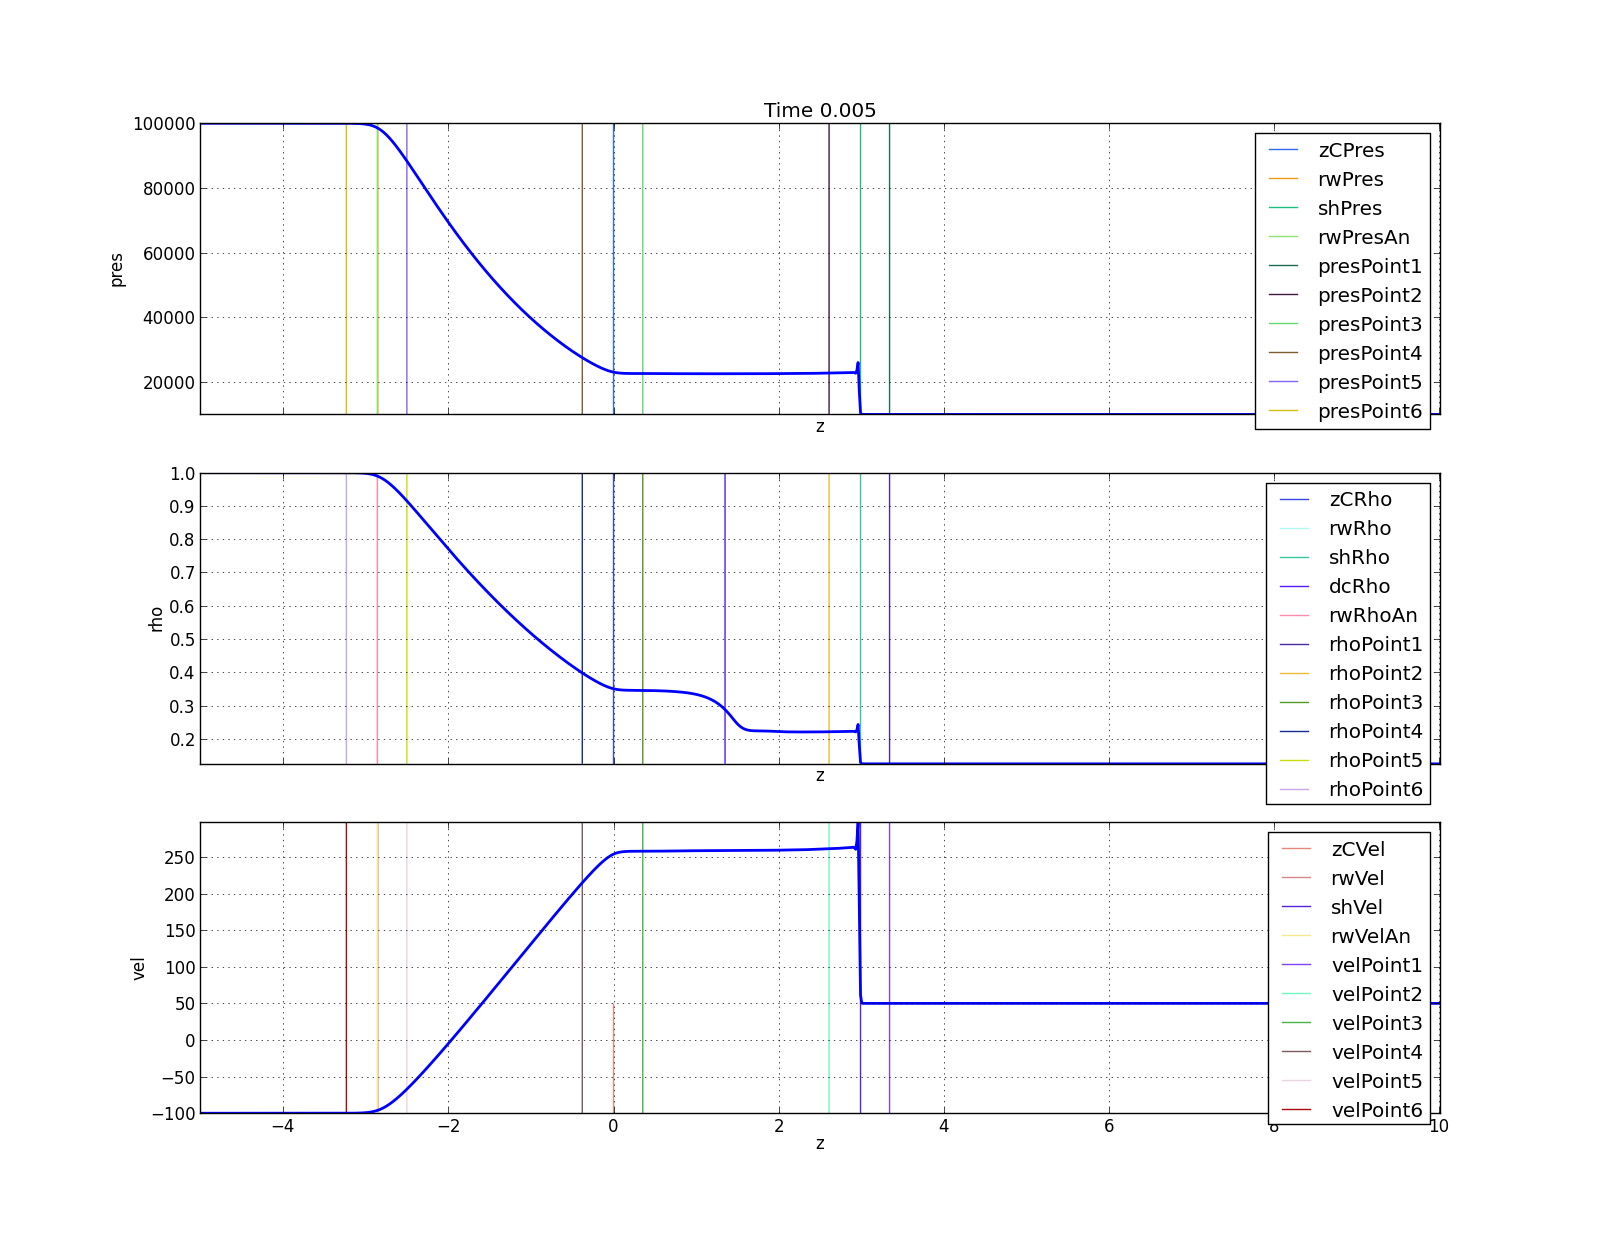
\includegraphics[scale=0.4]{complete.png}
 \label{Fig: 1}
	\caption{\emph{complete}}
\end{figure}

Observations:
\begin{enumerate}
\item csRW = cs6 - velLeft (this should always be true)
\item I don't know how to determine analytically csShock in this case when velocities are not 0(but I think there is a way), that's why shPointAn is not shown in the graph in this case. I could calculate csShock from empirical determination of shPoint (csShock = (shPoint - shPointPrevious) / dt) , but this not done yet(to compare with cs1 and cs2). Calculating csShock as sqrt(gamma * pres / rho) in shPoint is not practical because of the discontinuity and oscillations
\item relations fulfilled see out\_complete file
\item making velRight = -300 (greater than csShock) will make appear oscillations
\item But this was the case when velRight \textless 0 and velLeft \textgreater 0, when changing signs(fluids not approaching each other) this oscillation does not appear
\end{enumerate}

\begin{figure}[!h]
 \centering
 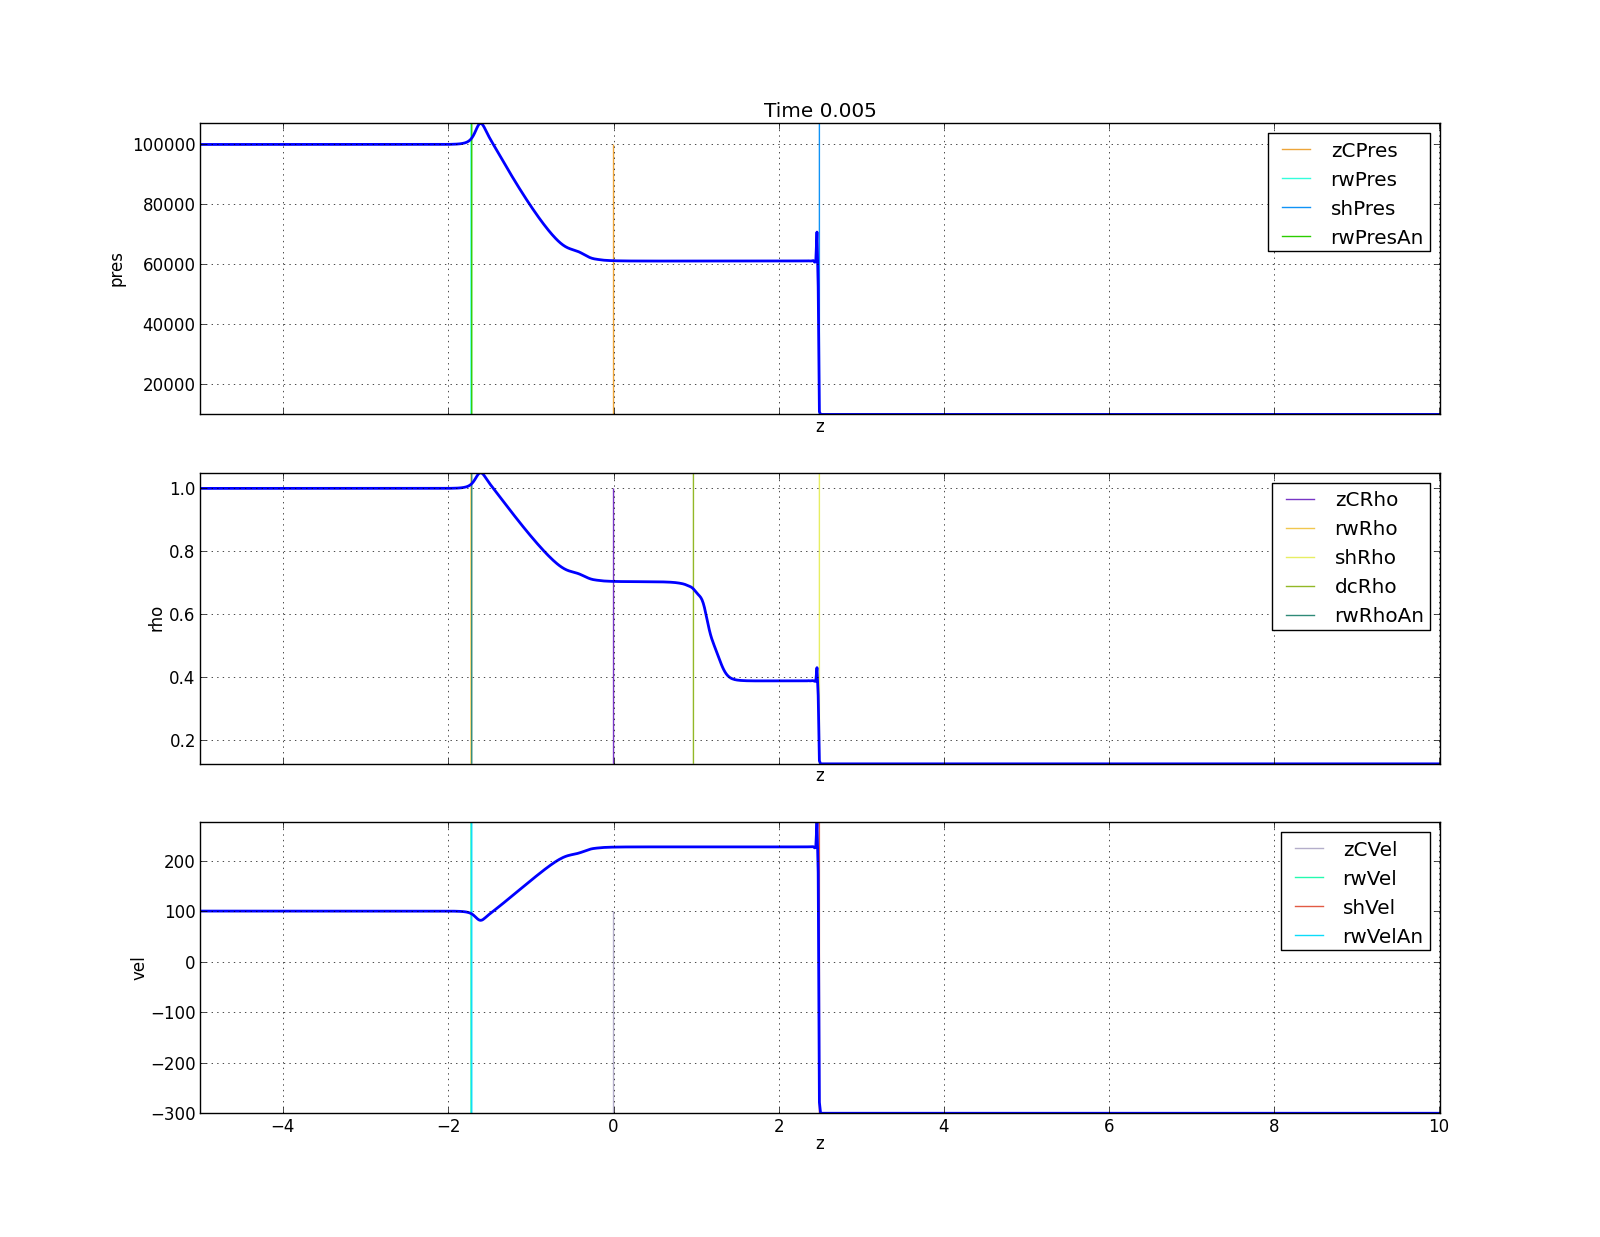
\includegraphics[scale=0.4]{complete300.png}
	\caption{\emph{complete abs(velRight) bigger}}
 \label{Fig: 1}
\end{figure}


\section*{Expansion into vacuum}

Case a
\begin{figure}[!h]
 \centering
 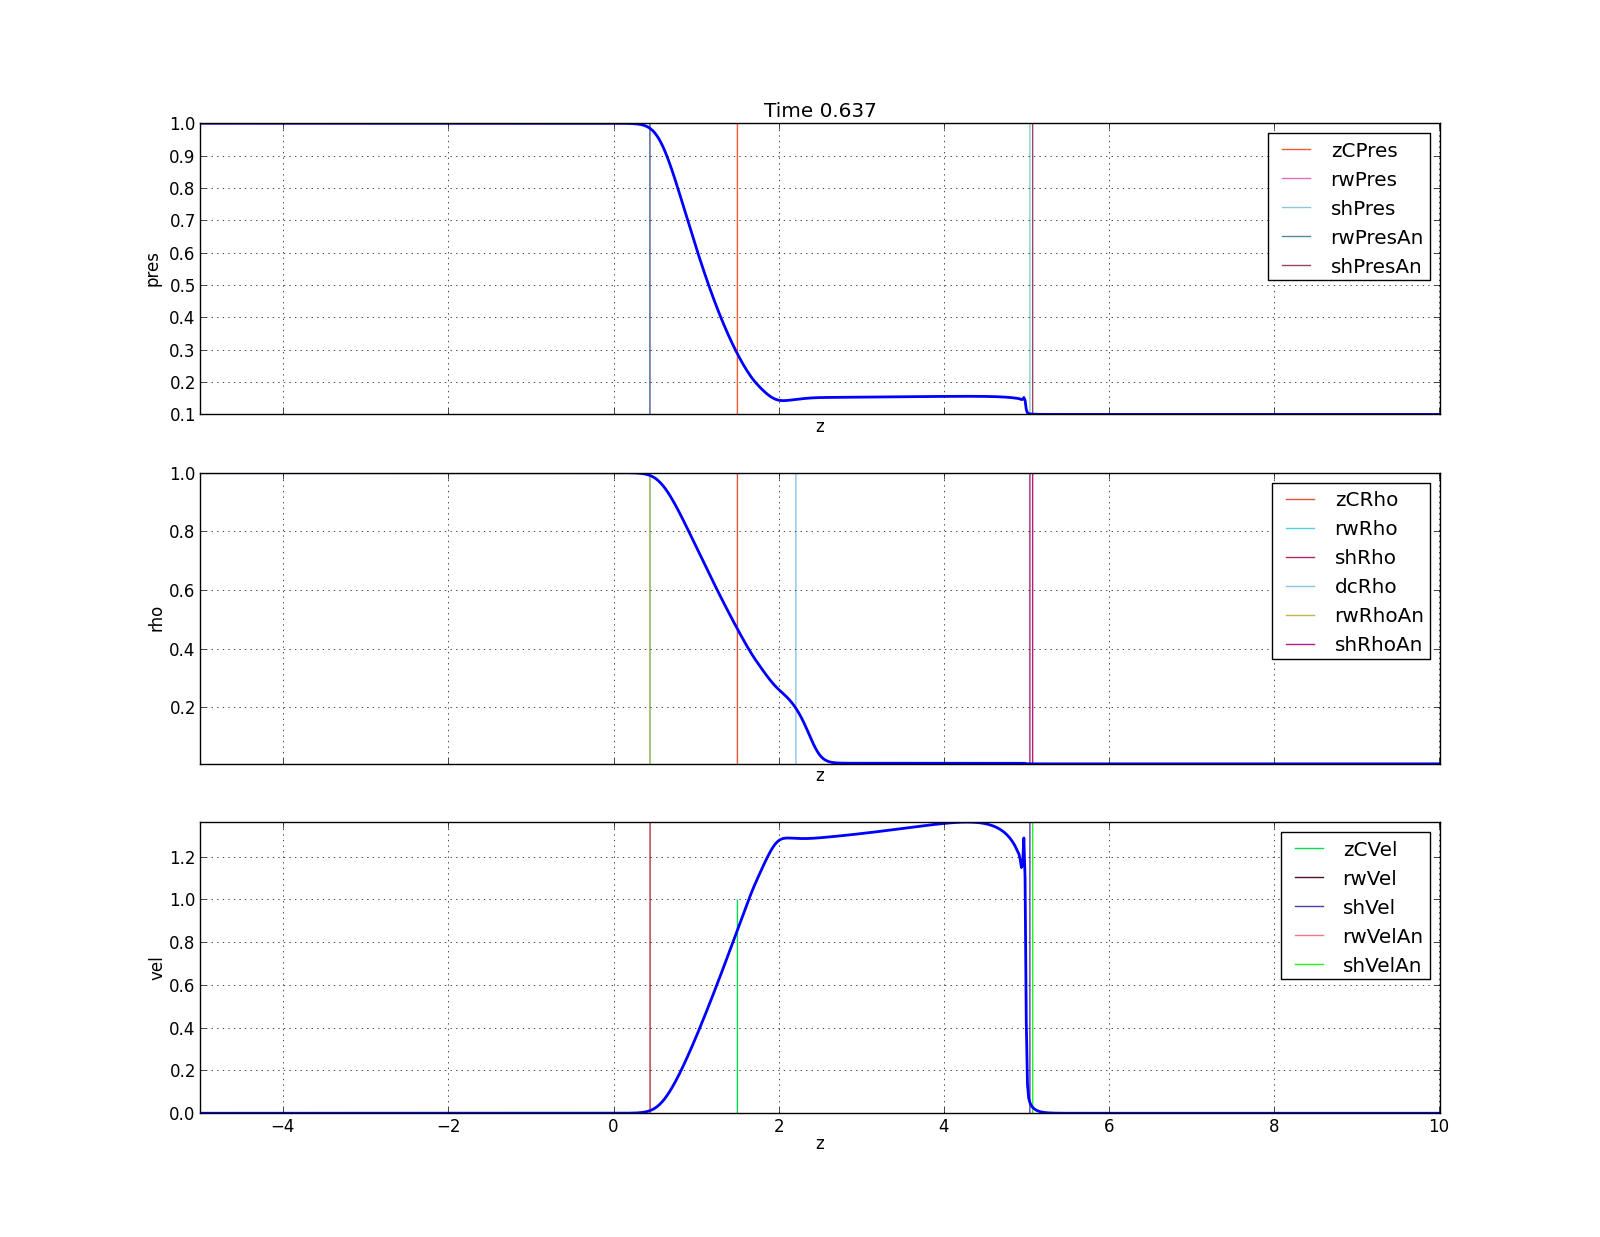
\includegraphics[scale=0.4]{exp_vacuum_a.png}
	\caption{\emph{exp vacuum case a}}
 \label{Fig: 1}
\end{figure}


Case b

\begin{figure}[!h]
 \centering
 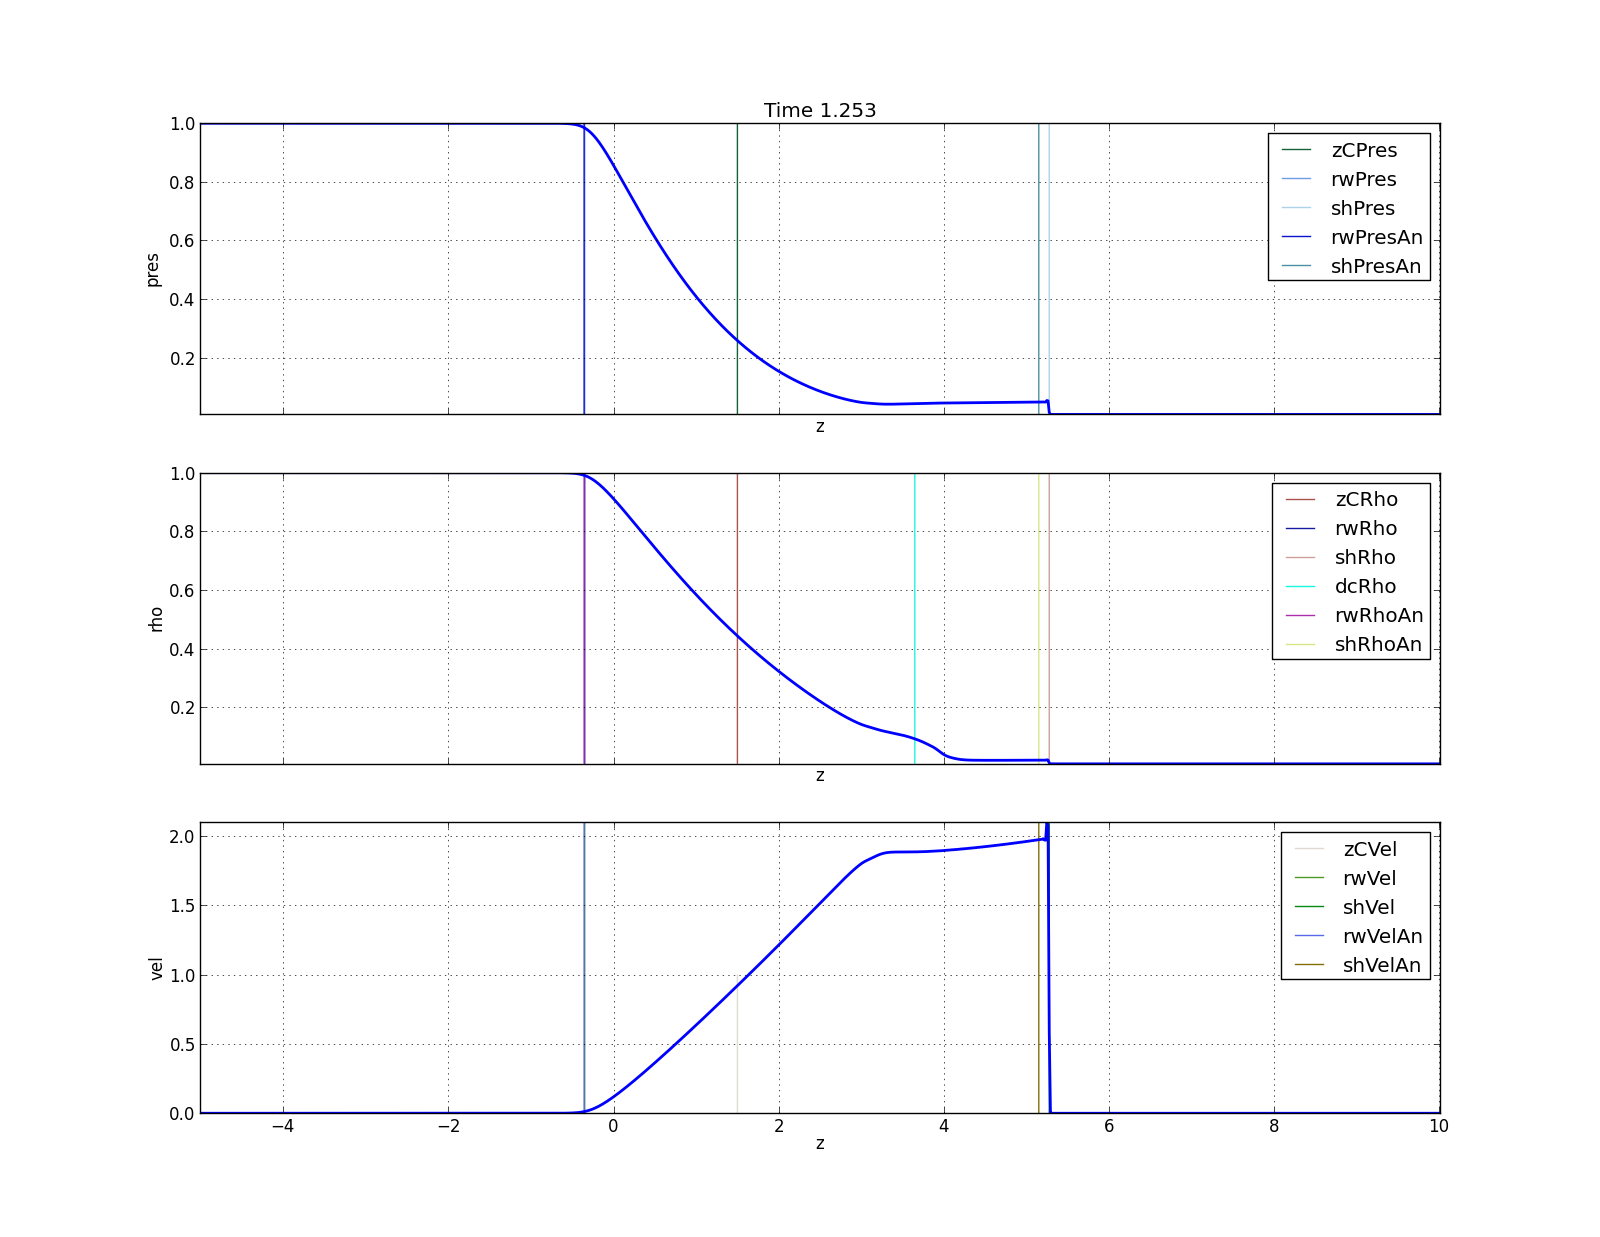
\includegraphics[scale=0.4]{exp_vacuum_b.png}
	\caption{\emph{exp vacuum case b}}
\end{figure}

Observations:
\begin{enumerate}
\item fluid from left is not filling instantly the right side
\item velocity grows slower in case b
\item density falls faster in case a 	- because of low density shPointAn is not very well calculated
\end{enumerate}

\section*{TODO}

\begin{enumerate}
\item move legend out of the plot
\item calculate shPoint velocity (csShock) in case of complete problem (I don't know the analyitical solution in this case)	
\end{enumerate}
\end{document}

